\chapter{Single dimension experiments}

\todo[inline]{
    Elaboration of this part based on the trained single dimension models.
}

\section{Reference model}

\section{Single dimension weakly supervised models}

\subsection{Evaluation of the model Hyperparameters}

\subsubsection{Weighted vs. unweighted point loss performance}

Contrary to fully supervised models, in the weakly supervised case, the ratio between labelled points is not as unbalanced.
This explains the weighted point loss performance compared to the unweighted point loss performance.

\begin{SCfigure}[][htb]
    \centering
    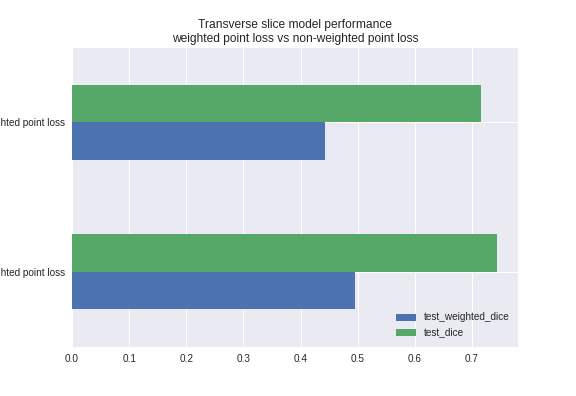
\includegraphics[width=.95\textwidth]{images/TransverseModel_weightedvsnonweighted.png}
    \caption{Illustration of the difference in model performance between a weighted point loss function and the unweighted point loss function}
\end{SCfigure}

\subsubsection{Value of the added loss components}

The added loss compontents show to deliver some added value.

\begin{SCfigure}[][htb]
    \centering
    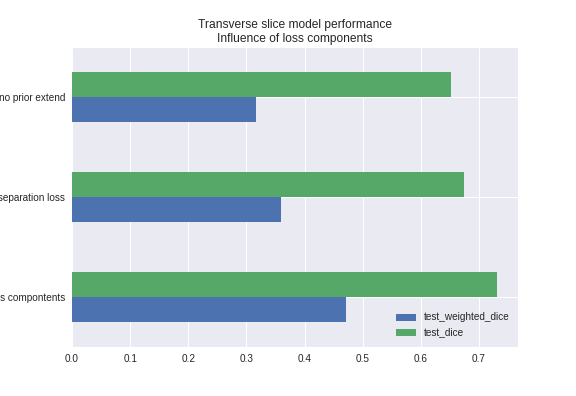
\includegraphics[width=.95\textwidth]{images/TransverseModel_Losscomponents.png}
    \caption{Evaluation of the added value of loss components}
\end{SCfigure}

\subsection{Evolution of the model performance with increased labelling effort}